% Idee: ???
% Tekst: ???
% Tõlge: Ahto Truu

\documentclass[a4paper,11pt]{article}
\usepackage[ru]{../../eio}

\usepackage{tikz}
\tikzset{every picture/.style = {thick, scale=0.5}}
\tikzset{uno/.style = {fill, shape=circle, inner sep=2}}
\tikzset{post/.style = {fill, shape=circle, inner sep=1}}
\tikzset{label/.style = {black, midway}}

\begin{document}

\begin{ol}{\eio}{\vv 19.04.2020}{\yle}{}
\begin{yl}{1}{Забор}{aed}{1 сек / 3 сек}{100 очков}

Уно сторит забор вокруг пастбища. Забор имеет вид замкнутой ломанной, которая состоит из $N$ отрезков. То есть, каждый отрезок начинается с конца предыдущего, а конец последнего отрезка совпадает с началом первого. Отрезки пронумерованы $1 \ldots N$ против часовой стрелки. Можно предпологать, что отрезки не пересекаются и не касаются (кроме общих конечных точек последовательных отрезков).

По окончании работы, Уно хочет осмотреть результат. Напиши программу, которая по месту нахождения Уно установит, которые отрезки ему видны. Уно может находиться как внутри огороженной территории, так и снаружи, однако он не может находиться с каким-либо отрезком забора на одной прямой.

Отрезок забора виден, если найдётся такой отрезок, соединяющий место нахождения Уно с какой-то точкой отрезка забора, который бы не пересекался и не соприкасался с другими отрезками забора. (Другими словами, Уно должен видеть часть отрезка забора ненулевой длины.)

\sis В первой строке файла \sisf целое число $N$ ($3 \le N \le 1\,000$) --- количество отрезков забора. Во второй строке два разделённых пробелом целых числа --- координаты $X$ и $Y$ места нахождения Уно. В каждой из следующих $N$ строк два разделённых пробелом целых числа --- на строке $i + 2$ координаты $X_i$ и $Y_i$ начала отрезка номер $i$. Все координаты целые числа, модули которых не более $10^5$.

\val В первую строку файла \valf вывести целое число $M$ --- количество отрезков забора, видимых Уно. Во вторую строку вывести $M$ разделённых пробелами целых чисел --- номера видимых Уно отрезков забора в возрастающем порядке.

\begin{wrapfigure}[1]{r}{0.3\textwidth}
\vskip -20pt
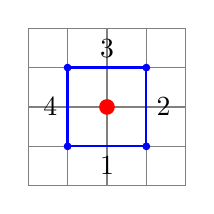
\begin{tikzpicture}
  \draw[gray, thin, step=1] (0, 0) grid (4, 4);
  \draw[blue] (1, 1)
    -- (3, 1) node[post]{} node[label, below]{1}
    -- (3, 3) node[post]{} node[label, right]{2}
    -- (1, 3) node[post]{} node[label, above]{3}
    -- (1, 1) node[post]{} node[label, left]{4};
  \fill[red] (2, 2) node[uno]{};
\end{tikzpicture}
\vskip 10pt
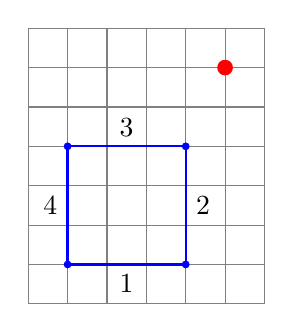
\begin{tikzpicture}
  \draw[gray, thin, step=1] (0, 0) grid (6, 7);
  \draw[blue] (1, 1)
    -- (4, 1) node[post]{} node[label, below]{1}
    -- (4, 4) node[post]{} node[label, right]{2}
    -- (1, 4) node[post]{} node[label, above]{3}
    -- (1, 1) node[post]{} node[label, left]{4};
  \fill[red] (5, 6) node[uno]{};
\end{tikzpicture}
\vskip 10pt
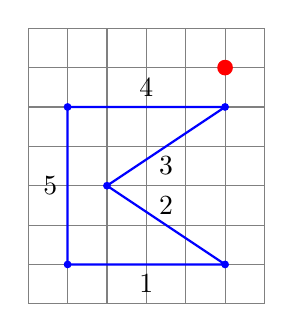
\begin{tikzpicture}
  \draw[gray, thin, step=1] (0, 0) grid (6, 7);
  \draw[blue] (1, 1)
    -- (5, 1) node[post]{} node[label, below]{1}
    -- (2, 3) node[post]{} node[label, above]{2}
    -- (5, 5) node[post]{} node[label, below]{3}
    -- (1, 5) node[post]{} node[label, above]{4}
    -- (1, 1) node[post]{} node[label, left]{5};
  \fill[red] (5, 6) node[uno]{};
\end{tikzpicture}
\end{wrapfigure}

\nde[0]{3cm}{3cm}

\nde[1]{3cm}{3cm}

\nde[2]{3cm}{3cm}

\hnd В этом задании тесты поделены на группы. За каждую группу очки получат только те решения, которые пройдут все тесты этой группы. В группах выполняются следующие дополнительные условия:
\begin{xenum}
  \item ($3 + 3$ очка) $N \le 50$ и забор имеет вид выпуклого многоугольника;
  \item ($7 + 7$ очков) забор имеет вид выпуклого многоугольника;
  \item ($2 + 5 + 5$ очков) $N \le 50$ и все отрезки забора параллельны координатным осьям;
  \item ($18$ очков) все отрезки забора параллельны координатным осьям;
  \item ($4 + 5 + 5$ очков) $N \le 50$;
  \item ($16$ очков) $N \le 200$;
  \item ($20$ очков) дополнительных условий нет.
\end{xenum}

\end{yl}
\end{ol}
\end{document}
